% TeX root=../main.tex

\section{Apresentação}

O eslavo antigo é uma língua morta, conhecida pelos textos do século X e XI\@.
Os textos eslavos antigos são quase todos textos religiosos traduzidos do grego
e não há literatura original em eslavo antigo.
Os únicos textos originais são inscrições, pouco numerosas, mas nos quais
formulação cristã é de origem grega.

O eslavo antigo foi a língua falada pelos eslavos dos Bálcãs orientais, no
território da atual Bulgária e Macedônia, o que faz com que ele por vezes seja
chamado de búlgaro antigo (\glsxtrshort{alemão}~\emph{Altbulgarisch}).
Uma outra denominação é aquela que não é mais utilizada em francês mas continua
em em uso em alemão em inglês, o eslavão antigo ou o eslavo eclesiástico antigo
(\glsxtrshort{alemão}~\emph{Altkirchenslavisch}, \glsxtrshort{inglês}~\emph{Old Church Slavonic}).
O eslavão (ou no caso os eslavões: eslavão russo, eslavão sérvio etc.), é a
língua litúrgica das igrejas ortodoxas russa, ucraniana, búlgara e sérvia e
representa uma continuação do eslavo antigo, adaptada superficialmente às
particularidades de cada uma das línguas eslávicas.
Neste sentido, as variantes modernizadas do eslavo antigo persistiram até que a
língua se tornasse morta, mas em um contexto extremamente restrito de uso
litúrgico.

Apontamos tradicionalmente o fim do eslavo antigo e a passagem ao búlgaro
moderno no fim do século XI\@.

\section{Notas históricas}

Os falantes dessa língua são divididos essencialmente em três grupos étnicos.
As tribos eslávicas chegam ao leste dos Balcãs ao fim do século V, sendo a
principal a dos severianos, que significa ``os do norte'' (outros severianos se
encontram no território), cf.~\autoref{fig:eslavos_sec8_9}.
Esses eslavos se instalam em um território ocupado por trácios que são
rapidamente assimilados.
Eles engajam em saques pelos Balcãs, quase chegando ao Peloponeso.
Por volta do meio do século VII, uma população asiática de origem
turco-mongólica, os búlgaros, chega e impõe sua dominação sobre os eslavos (isto
é, aos eslavos propriamente ditos e aos trácios eslavizados).

\begin{figure}[!htb]
  \begin{center}
    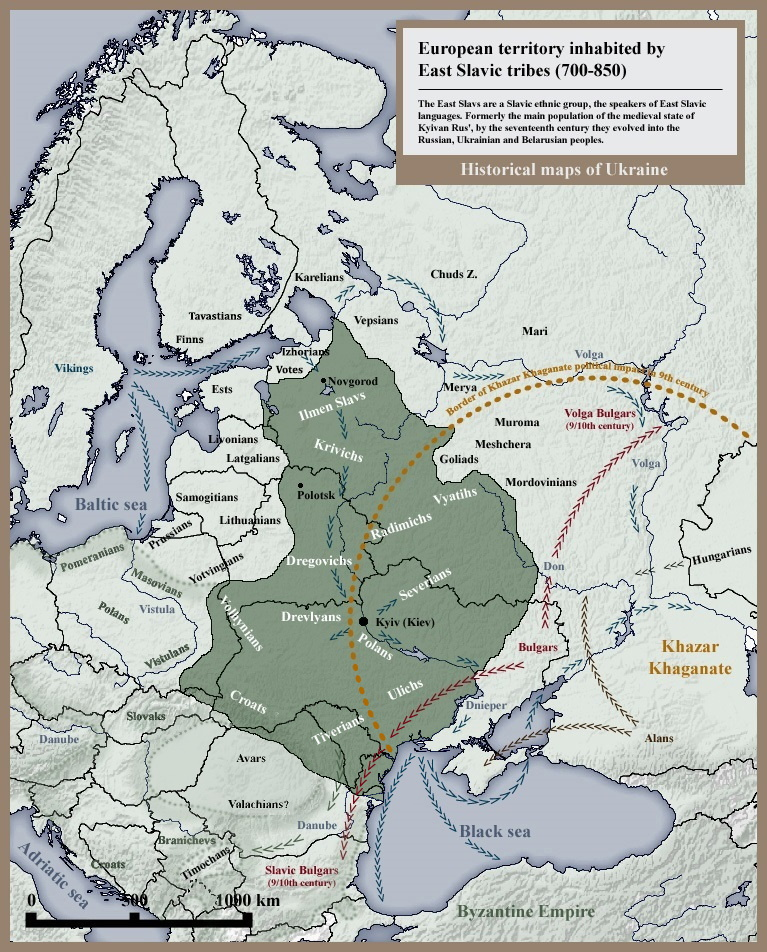
\includegraphics[width=0.75\textwidth]{assets/East_Slavic_tribes_peoples_8th_9th_century.jpg}
  \end{center}
  \caption{Eslavos durante os séculos VIII-IX\@. Fonte: \url{https://pt.wikipedia.org/wiki/Ficheiro:East_Slavic_tribes_peoples_8th_9th_century.jpg}}\label{fig:eslavos_sec8_9}
\end{figure}


A fundação do reino da Bulgária se segue à vitória do khan Asparuch sobre o
imperador bizantino Constantino IV em 680.
Esses búlgaros, que deram seu nome ao país, são rapidamente eslavizados por sua
vez.
Para evitar a confusão, chamamos a língua desse povo de ``proto-búlgaro'',
aparentada ao turco e separamos o termo ``búlgaro antigo'' à língua eslava, seja
como um equivalente ao ``eslavo antigo'' em sua totalidade, seja para designar o
dialeto búlgaro do eslavo antigo em oposição ao dialeto macedônio, o que será
útil aqui.

Em 862, o príncipe da Morávia (Chéquia atual), buscando aliança com Bizâncio para
se opor à crescente influência dos francos e da Igreja de Roma, pede ao
imperador bizantino Miguel III que envie missionários à Morávia.
Miguel incumbe dois monges de origem eslava da Tessalônica, Constantino (Cirilo
é seu nome de monge) e seu irmão Metódio de criar um alfabeto para o eslavo e
traduzir os evangelhos a essa língua. 
A missão na Morávia começa em 863.
Cirilo morre em 869, Metódio permanece na Morávia mas após sua morte em 885 seus
discípulos são perseguidos e se refugiam na Bulgária, que se torna o centro das
letras eslavas.

Um pouco antes deste momento, o reino da Bulgária, cuja capital é Pliska,
torna-se oficialmente cristão, em 864, com o batismo do rei Boris I (852--889).
O filho mais velho de Boris, Vladmir, o sucede brevemente, mas é deposto quatro
anos mais tarde.
Seu irmão Simeão (893--927) o sucede: inicialmente destinado a uma vida
monástica, Simeão é um letrado perfeitamente helenizado que havia estuado dez
anos em Constantinopla.
Ele move a capital para Preslav (Preslav Veliki ou Grande Preslav) desde o
início de seu reinado.
Aproveitando a presença dos discípulos de Cirilo e Metódio expulsos da Morávia
(885), Simeão torna Preslav em um centro cultural importante, onde a atividade
de cópia e tradução de textos gregos estava em pleno vapor.
Simeão se encarrega de favorecer o desenvolvimento das letras eslavas, afirmando
o prestígio de seu reino e firmando sua independência política frente a
Bizâncio: a Igreja búlgara se torna autônoma com relação à hierarquia grega,
depois autocéfala a partir de 915, e Simeão toma o título de imperador
(\ocsex{cEsar'I}) em 913.
Sob seu regime, o reino da Bulgária alcança seu apogeu e se estende desde o Mar
Negro ao Adriático (\emph{cf.}~\autoref{fig:reino_bulgaria})
Sob o sucessor de Simeão, seu filho Pedro I (927--969), a agitação social toma o
reino.
Após uma revolta na Macedônia ao final do século X, uma nova dinastia se instala
com o rei Samuel (976--1014), que move o centro de poder à Macedônia, na direção
do sudeste, e faz de Ohrid sua capital.
Mas o reino é subjugado por Bizâncio em 1014 e o imperador Basílio II ganha o
sobrenome de Bulgarotóctone.
Samuel morre um pouco depois da derrota.
Um  segundo reino da Bulgária se reconstitui no final do século XII (1186) e
tem por capital Tărnovo, que durará até a conquista turca em 1393.
Esse segundo reino da Bulgária corresponde ao período búlgaro moderno e a língua
desta época ja não é mais o eslavo antigo.

\begin{figure}[!htb]
  \begin{center}
    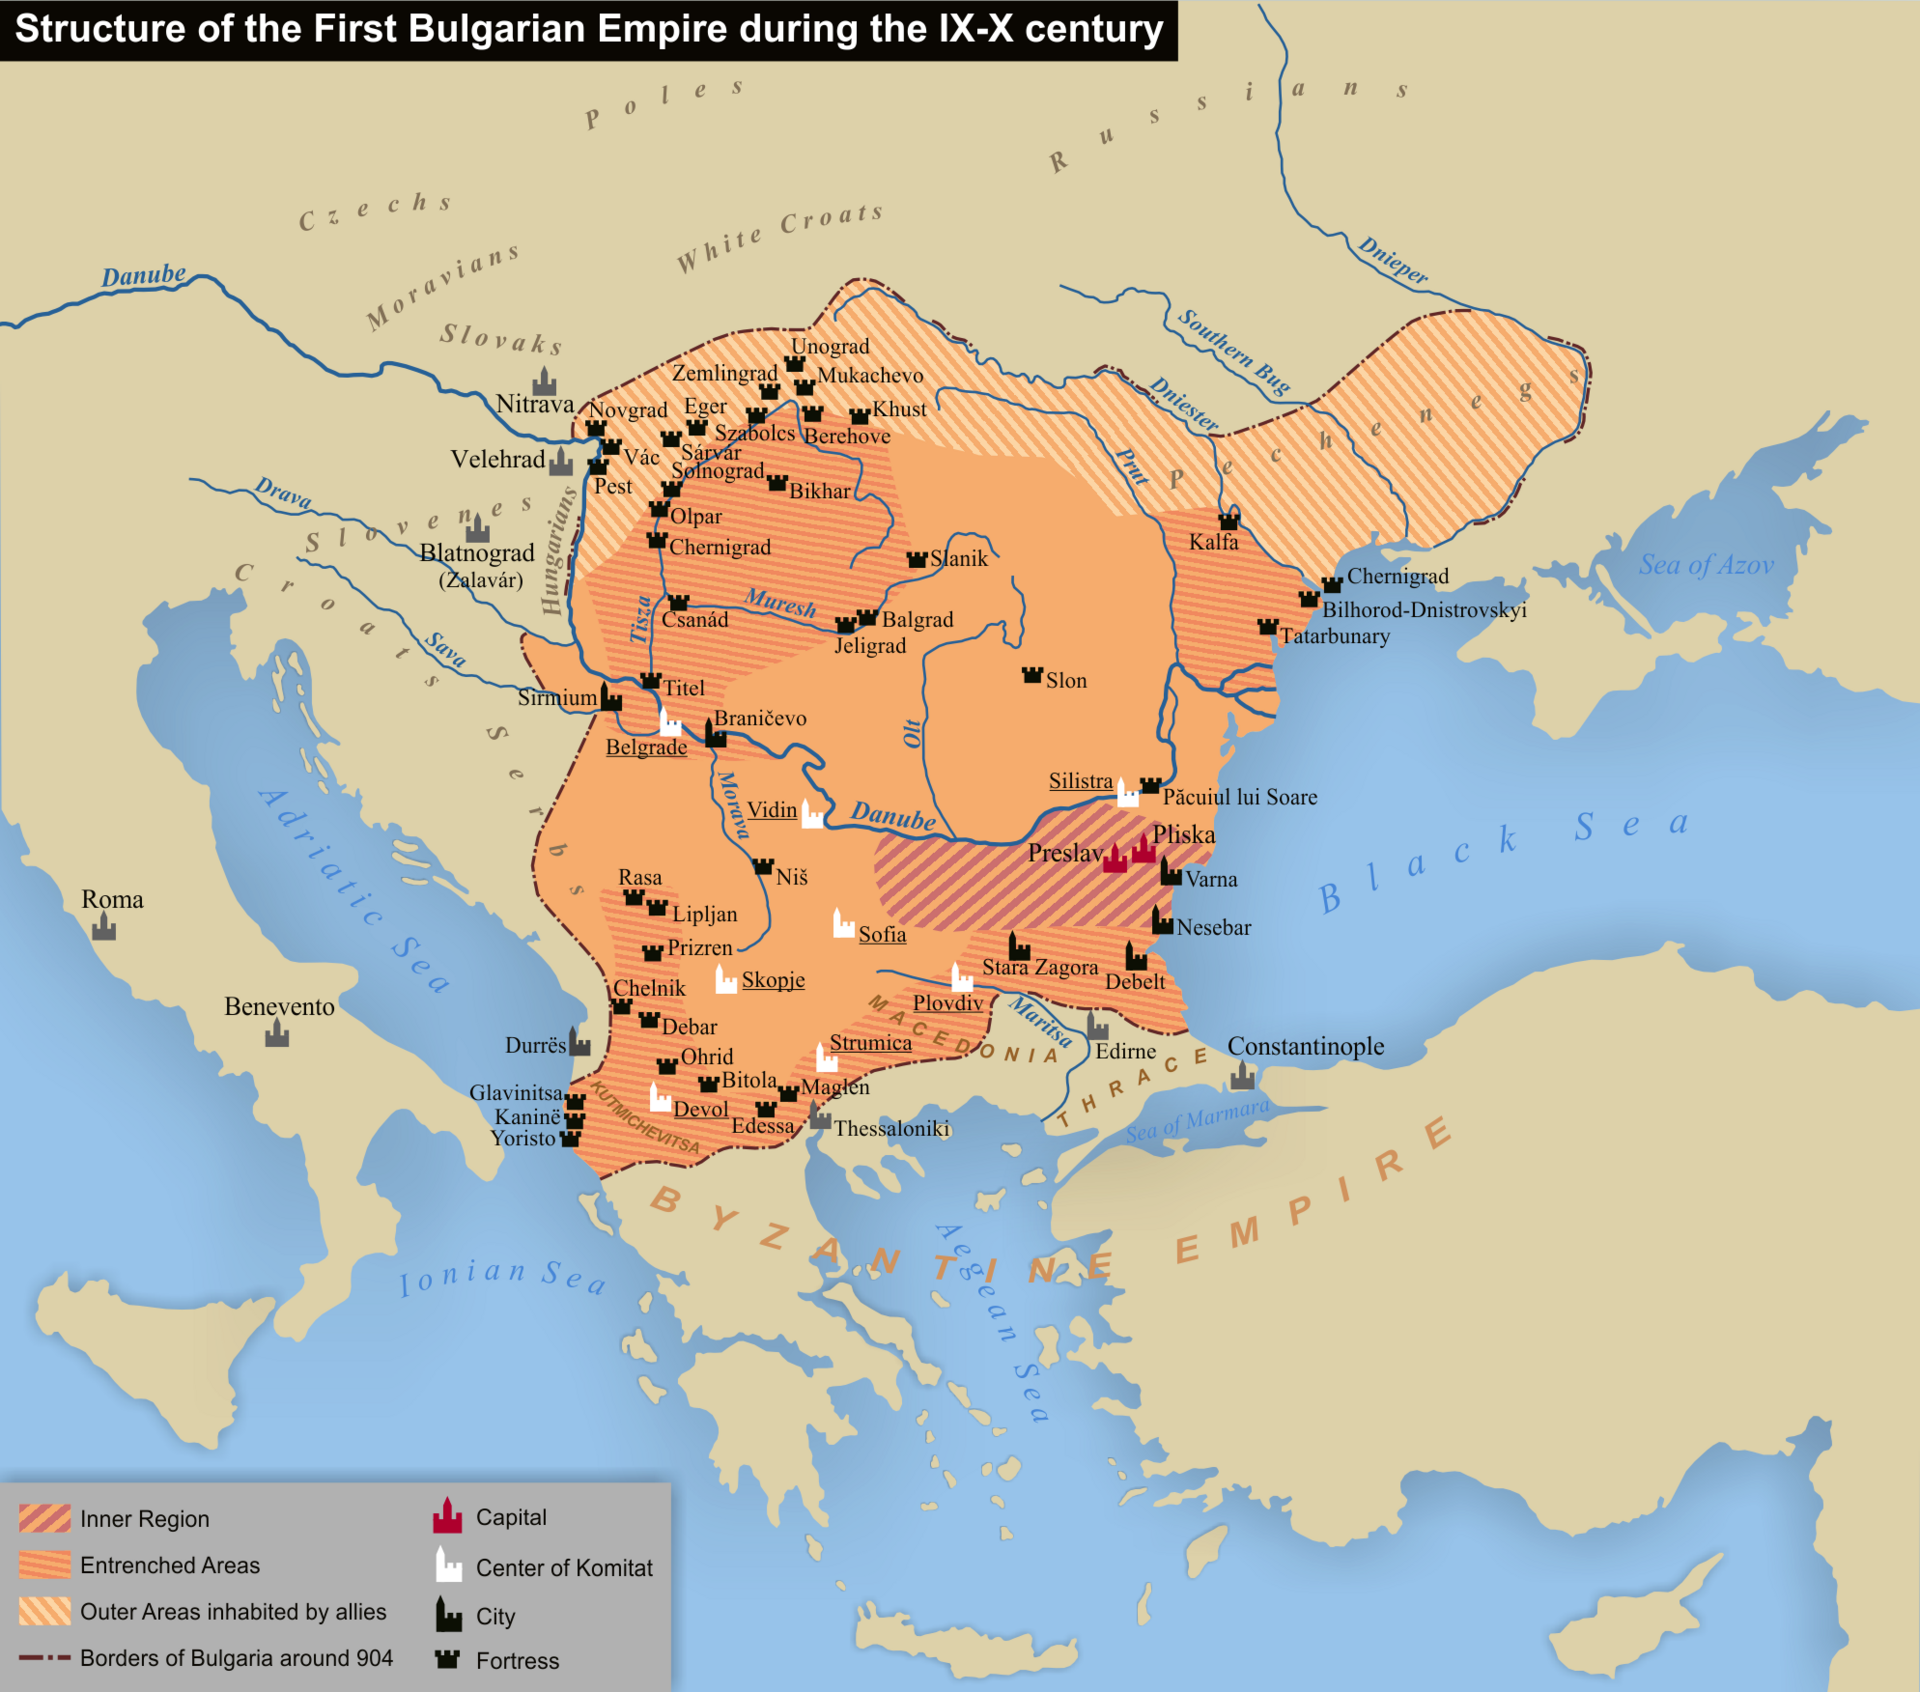
\includegraphics[width=0.75\textwidth]{assets/Structure_of_the_First_Bulgarian_Empire_during_the_IX-X_century.png}
  \end{center}
  \caption{Primeiro reino búlgaro. Fonte: \url{https://commons.wikimedia.org/wiki/File:Structure_of_the_First_Bulgarian_Empire_during_the_IX-X_century.png}}\label{fig:reino_bulgaria}
\end{figure}

\section{Grafia}

O eslavo antigo é grafado com dois alfabetos diferentes, que se sucedem e que
coexistiram durante um certo tempo (ver~\autoref{tab:alfabetos}).
O primeiro, inventado por Constantino-Cirilo segundo a tradição, é o alfabeto
glagolítico (também chamado glagolito), nome que, tal como cirílico para o outro
sistema, é tardio.
É um sistema único que não corresponde a qualquer outro sistema alfabético
contemporâneo conhecido.
As fontes do alfabeto glagolítico são disputadas.
Para alguns, trata-se de uma criação \emph{ex nihilo} de Cirilo, enquanto para
outros ele seria inspirado na escrita siríaca e para outros ainda essa escrita
seria derivada da cursiva grega.
Essa última tese, a mais difundida, tem voltado a ser favorecida~\cite[para o estado
da questão, ver][]{Marti2004}.
Não temos nenhum traço de escrita eslava antes de Cirilo, mas o alfabeto grego
era utilizado para representar o eslavo, de modo que a vemos em algumas
inscrições, e é possível que Cirilo não tenha feito nada se não dar a forma
definitiva a um sistema esboçado por outros.
A escrita glagolítica continua sendo usada na Croácia até o começo do século XX
em uma variante conhecida por ``glagolito quadrado'', por conta do formato de
suas letras.

Noutras regiões, ela é no entanto rapidamente abandonada e substituída por um
outro sistema, o alfabeto chamado cirílico (mesmo ele não sendo invenção de
Cirilo mas de seus sucessores), derivado da uncial grega.
Os fonemas que fossem idênticos em eslavo e em grego são notados pela letra
grega correspondente: por isso das vogais \emph{a}, \emph{e}, \emph{i},
\emph{o}, os dois últimos fonemas são notados por dois grafemas diferentes,
transpondo a situação do grego: 
\grafema{{\rus{}Ꙇ}} e \grafema{{\rus{}И}} para /i/ (grego \grafema{Ι} e
\grafema{Η}, pronunciado [i] por causa do iotacismo), \grafema{{\rus{}О}} e
\grafema{{\rus{}Ѡ}} para /o/, enquanto para \emph{u} há a notação
\grafema{{\rus{}ОУ}}, calque do dígrafo grego \grafema{ΟΥ};
os dois grafemas para /i/ e /o/ existem igualmente em glagolítico e o grafema
para /u/ em glagolítico é claramente uma ligatura em que o primeiro elemento é o
grafema para /o/, o que advoga em favor da tese de que o alfabeto glagolítico
seja derivado do grego.
De mesma maneira, a maior pare das consoantes do cirílico conservam a forma de
seu modelo grego.
A notação de fonemas que não teriam correspondente em grego (por exemplo as
fricativas \emph{š}, \emph{ž}, \emph{č}, a africada \emph{c} e as vogais nasais
\emph{ę} e \emph{ǫ}) se faz por meio de grafemas do alfabeto glagolítico.


\begin{table}[!htb]
  \caption{Alfabetos cirílico e glagolítico}\label{tab:alfabetos}
  \begin{center}
    \begin{tabular}[c]{llll||llll}
      \toprule
      glagolítico & cirílico & translit. & IPA & glagolítico & cirílico &
      translit. & IPA\\
      \midrule
      {\ocs{}Ⰰ}   & {\rus{}А} & a  & [a]   & {\ocs{}Ⱆ} & {\rus{}ОУ Ꙋ}  & u    & [u]\\
      {\ocs{}Ⰱ}   & {\rus{}Б} & b  & [b]   & {\ocs{}Ⱇ} & {\rus{}Ф}     & f    & [f]\\
      {\ocs{}Ⰲ}   & {\rus{}В} & v  & [v]   & {\ocs{}Ⱈ} & {\rus{}Х}     & x    & [x]\\
      {\ocs{}Ⰳ}   & {\rus{}Г} & g  & [g]   & {\ocs{}Ⱌ} & {\rus{}Ц}     & c    & [ts]\\
      {\ocs{}Ⰴ}   & {\rus{}Д} & d  & [d]   & {\ocs{}Ⱍ} & {\rus{}Ч}     & č    & [tʃ,]\\
      {\ocs{}Ⰵ}   & {\rus{}Є} & e  & [ʲe]  & {\ocs{}Ⱎ} & {\rus{}Ш}     & š    & [ʃ,]\\
      {\ocs{}Ⰶ}   & {\rus{}Ж} & ž  & [ʒ]   & {\ocs{}Ⱋ} & {\rus{}щ}     & št   & [ʃt,]\\
      {\ocs{}Ⰷ}   & {\rus{}Ѕ} & dz & [dz,] & {\ocs{}Ⱏ} & {\rus{}Ъ}     & ŭ, ъ & [ə]\\
      {\ocs{}Ⰸ}   & {\rus{}З} & z  & [z]   & {\ocs{}ⰟⰊ } & {\rus{}Ꙑ ЪИ}     & y    &\\
      {\ocs{}Ⰹ Ⰺ} & {\rus{}И} & i  & [i]   & {\ocs{}Ⱐ} & {\rus{}Ь}     & ĭ    & [ʲe]\\
      {\ocs{}Ⰻ}   & {\rus{}Ꙇ} & i  & [i]   & {\ocs{}Ⱑ} & {\rus{}Ѣ}     & ě    & [ʲa]\\
      {\ocs{}Ⰼ}   & {\rus{}Ћ} & g' & [g,]  & {\ocs{}Ⱓ} & {\rus{}Ю}     & ju   & [ju]\\
      {\ocs{}Ⰽ}   & {\rus{}К} & k  & [k]   & {\ocs{}}  & {\rus{}Ꙗ}     & ja   & [ja]\\
      {\ocs{}Ⰾ}   & {\rus{}Л} & l  & [l]   & {\ocs{}}  & {\rus{}Ѥ}     & je   & [je]\\
                  & {\rus{}Л҄} & l' & [l']  & {\ocs{}Ⱔ} & {\rus{}Ѧ}     & ę    & [ɛ̃]\\
      {\ocs{}Ⰿ}   & {\rus{}М} & m  & [m]   & {\ocs{}Ⱗ} & {\rus{}Ѩ}     & ję   & [jɛ̃]\\
      {\ocs{}Ⱀ}   & {\rus{}Н} & n  & [n]   & {\ocs{}Ⱘ} & {\rus{}Ѫ}     & ǫ    & [ɔ̃]\\
                  & {\rus{}Н҄} & n' & [n,]  & {\ocs{}Ⱙ} & {\rus{}Ѭ}     & jǫ   & [jɔ̃]\\
      {\ocs{}Ⱁ}   & {\rus{}О} & o  & [ɔ]   & {\ocs{}Ⰰ} & {\rus{}Ѯ}     & ks   & [ks]\\
      {\ocs{}Ⱂ}   & {\rus{}П} & p  & [p]   & {\ocs{}Ⰰ} & {\rus{}Ѱ}     & ps   & [ps]\\
      {\ocs{}Ⱃ}   & {\rus{}Р} & r  & [r]   & {\ocs{}Ⱚ} & {\rus{}Ѳ}     & t    & [t]\\
                  & {\rus{}Р҄} & r' & [r,]  & {\ocs{}Ⱛ} & {\rus{}Ѵ}     & u    & [u]\\
      {\ocs{}Ⱄ}   & {\rus{}С} & s  & [s]   & {\ocs{}Ⱉ} & {\rus{}Ѡ}     & o    & [o]\\
      {\ocs{}Ⱅ}   & {\rus{}Т} & t  & [t]   &  &  &   &    \\
      \bottomrule
    \end{tabular}
  \end{center}
\end{table}

Como em grego, as letras possuem também um valor numérico.
No alfabeto glagolítico, o valor segue a ordem das letras (\grafema{a} = 1,
\grafema{b} = 2, \grafema{v} = 3, \grafema{g} = 4, etc), mas no alfabeto
cirílico o valor é calcado naquele da letra grega, de modo que há um salto de
uma unidade com relação ao valor numérico do glagolítico (assim, é
{\rus{}В}\slash{}\emph{v} que vale 2, e não {\rus{}Б}\slash{}\emph{b}, que não possui valor
numérico, {\rus{}Г}\slash{}\emph{g} = 3, etc.).

Nos manuscritos tanto em glagolítico como em cirílico, o uso de abreviações para
palavras comuns, à imitação do grego, é constante: a abreviação é sinalizada
pelo \emph{titulus}, um sinal \grafema{{\rus{} ҃  }}, colocado acima da palavra abreviada.

O alfabeto cirílico, que é assim um alfabeto misto, deve ter se formado no
contexto bilíngue dos eslavos helenizados.
Seus primeiro traços epigráficos datam do século X\@: a mais antiga inscrição em
cirílico é datada de 921.
A sua simplicidade e o prestígio que lhe conferia seu modelo grego garantiram
seu sucesso e logo foram refeitas cópias em que se transcrevia em cirílico os
antigos manuscritos em glagolítico.
É difícil dizer se ocorreu uma política deliberada para impor o alfabeto
cirílico: no máximo pode-se concluir a partir do celo do rei Pedro (morto em
969) e da inscrição de Samuel de 993, ambos em cirílico, que os soberanos eles
mesmos, ao utilizarem o alfabeto cirílico como alfabeto oficial em alguma
medida, contribuíram para sua propagação.
No entanto, os tradutores e copistas da escola de Ohrid mantiveram o uso do
glagolítico.
A maior parte dos textos eslavos antigos conservados estão em glagolítico (ver
abaixo), o que se explica pelo fato de que nos foram conservados sobretudo os
texto do período macedônio, da escola de Ohrid.
Nas inscrições de Preslav dos séculos IX e X, os dois sistemas coexistem.

Fora dos Balcãs, encontram-se algumas inscrições glagolíticas na Rússia, em Santa
Sofia de Kiev e em Novgorod, mas elas são muito pouco numerosas e o cirílico que
se impõe desde os primeiros textos.
Por outro lado, o \emph{Codex de Novgorod} ou \emph{Saltério de Novgorod} (três
tabuletas de madeira cobertas por cera com quatro faces inscritas), descoberto
em 2000 (e que por isso não são listados em \textcite{Schenker1995} nem em
\textcite{BirnbaumSchaeken1999}), fragmento de um saltério em eslavo antigo,
está em cirílico: data-se eles do primeiro quarto do século XI e eles assim se
juntam aos documentos mais antigos em eslavo antigo conservados (edição
provisória de A.~A.\ Zalizniak e V.~L.\ Janin em \emph{Voprosy Jazykoznanija}
(2001/5: 3--25)).
O texto difere ligeiramente daquele do \emph{Saltério do Sinai}, o que atesta
duas tradições eslavas distintas.
Na medida em que o texto não provém da região da Bulgária\hyp{}Macedônia, mas
foi escrito por um russo e apresenta assim alguns traços do eslavo oriental, não
o incluiremos à lista de textos em eslavo antigo canônicos.

\section{Documentos}

O corpus eslavo antigo \emph{stricto sensu} é constituído por um número limitado
de textos de extensão desigual, que constituem o ``cânone'' ao qual se somam
algumas inscrições conservadas.
Encontrar-se-á uma descrição dos textos e das edições modernas
em~\textcite[87--130]{BirnbaumSchaeken1999}, que integra os documentos
descobertos depois da publicação do \emph{Manuel du vieux slave} de Vaillant.

\subsection{O cânone clássico}

\begin{compactitem}[--]
    \item \emph{Folhas de Kiev} (ou \glsxtrlong{Kiev}) [\glsxtrshort{Kiev}],
      fragmento de missal seguindo o rito romano, traduzido do latim, em eslavão
      morávio (7 fol., glagol., séc.\ X),
      é o texto mais antigo e conservado e o único que atesta diretamente a
      tradição morávia. Ed. J. Schaeken, \emph{Die Kiever Blätter}, Amsterdam, 1987.
    \item \glsxtrlong{Zogr} [\glsxtrshort{Zogr}], quatro evangelhos (270 fol.,
      glagol., final do séc.\ X--começo do XI, Macedônia, provavelmente o manuscrito
      mais antigo conservado depois do 
      \glsxtrlong{Kiev}). Ed. V. Jagic, \emph{Quattuor evangeliorum codex
      glagoliticus olim Zographensis nunc Petropolitanus}, Berlim, 1879
      (transcrição cirílica).
    \item \glsxtrlong{Marianus} [\glsxtrshort{Marianus}], quatro evangelhos (171 + 2 fol., faltam os
      capítulos de 1 a 5 e 24 de Mateus, glagol., final do séc.\ X--começo do
      XI, Macedônia, provavelmente posterior ao \glsxtrshort{Zogr}). Ed. V. Jagic,
      \emph{Mariinskoe četveroevangelie, s primečanijami i s priloženijami}, S.
      Petersburgo 1883 (transcrição cirílica, glossário, aparato crítico com
      leituras divergentes de \glsxtrshort{Zogr}, \glsxtrshort{Assemanius}, \glsxtrshort{Sav} e do
      \emph{Evangelho de Ostromir}).
    \item \glsxtrlong{Assemanius} [\glsxtrshort{Assemanius}], evangeliários (158 fol., glagol.,
      XI, Macedônia). Ed. J. Vajs, J. Kurz, \emph{Evangeliář Assemanuv, Kodex
      Vatikánský 3.\ slovanský}, Praga, 1929-1955 (fac-símile, transcrição cirílica).
    \item \glsxtrlong{Sav} [\glsxtrshort{Sav}], evangeliário (130 fol., ciríl., XI°,
      Bulgária). Ed. O.~A.\ Knjazevskaja \emph{et al.}, \emph{Savvina kniga,
      drevneslavjanskaja rukopis’ XI, XI- XII i konca XIII veka}, Moscou, 1999 —
      (vol.\ 1: fac-símile, texto, comentários).
    \item Palimpsesto do Vaticano, fragmento de evangeliário (93 fol., ciríl.,
      final do séc.\ X--começo do XI, Bulgária). Ed. T. Kraštanov \emph{et al.},
      \emph{Vatikansko evangelie. Starobălgarski kirilski aprakos ot X.\ v.\ v
      palimpsesten Kodeks Vat.\ Gr.\ 2502}, Sofia, 1996 (apenas texto).
    \item \emph{Folhas de Ohrid}, fragmento de evangeliário e de lecionário (2
      fol., glagol., XI, Macedônia). Ed. T.~A.\ Lysaght, \emph{A selection of
      ancient Slav literary monuments incorporating Monumenta minora palaeobulgaricae}, Vienne 1982 (transcrição cirílica, fac-símile).
    \item \emph{Fragmento do Sinai}, fragmento de evangeliário (1 fol., glagol.,
      segunda metade do século XI). Ed.\ M. Altbauer, V. Mareš, ``Fragmentum
      glagoliticum evangeliarii palæoslovenici in codice Sinaitico 39
      (palimpsestum)'', Viena, 1980 (transcrição cirílica, fac-símile); com
      complementos dos mesmos em \emph{Wiener Slawistischer Almanach} 7, 1981.
    \item \emph{Saltério do Sinai} [\emph{Ps.}] (209 fol., glagol., XI,
      Macedônia). Ed.\  I.~C.\ Tarnanidis, \emph{The Slavonic manuscripts
      discovered in 1975 at St Catherine's Monastery on Mount Sinai},
      Tessalônica 1988 (para a primeira parte do manuscrito), F. Mareš,
      \emph{Psalterii Sinaitici pars nova}, Viena, 1997 (para a segunda parte)
      (introdução, transcrição cirílica, aparato crítico, concordância).
    \item \emph{Euchologe do Sinai} [\emph{Euch.}] (133 + 1 fol., glagol., XI,
      Macedônia). Ed.\ J. Frèek, \emph{Euchologium Sinaiticum. Texte slave avec
      sources grecques et traduction française}, Paris 1933-1939 (transcrição
      cirĺica, texto grego, tradução francesa); R. Nahtigal, \emph{Euchologium
      Sinaiticum. Starocerkvenoslovanski rlagoiski spomenik}, Ljubljana,
      1941-1942 (transcrição cirílica, fac-símile, glossário).
    \item \emph{Missal do Sinai} (80 fol., glagol, XI, Macedônia?). Ed.\ edição
      parcial, Tarnanidis 1988 (\emph{cf}.\ \emph{Saltério}).
    \item \glsxtrlong{Supr} [\glsxtrshort{Supr}], menólogo de \emph{mars} e
      homilías (118 + 16 + 151 fol., ciríl., XI, Bulgária), um dos manuscritos
      mais recentes, posterior a \glsxtrshort{Sav} Ed.\ J. Zaimov, M. Capaldo,
      \emph{Suprasǎlski ili Retkov sbornik}, Sofia, 1982--1983 (fac-símile,
      comentário, texto grego).
    \item \glsxtrlong{Clozianus} [\glsxtrshort{Clozianus}], fragmento de homiliário (12 + 2 fol.,
      glagol., XI, Macedônia). Ed.\ Dostál 1959 (transcrição cirílica e latina,
      texto grego e latino, tradução checa, fac-símile, glossário).
    \item \emph{Folhas de Rila} (1 + 6 fol., glagol., XI, Macedônia). Ed.\ I.\
      Gotev, \emph{Rilski glagoliceski listove}, Sofia, 1956 (transcrição
      cirílica, fac-símile, glossário).
    \item \emph{Folhas de Hilandar}, fragmento de Cirilo de Jerusalém (2 fol.,
      ciríl., XI, Bulgária). Ed. Lysaght 1982 (texto e fac-símile) (\emph{cf.}
      \emph{Folhas de Ohrid} acima).
    \item \emph{Folhas do Zograph}, fragmento de Basílio de Cesareia (2 fol.,
      ciríl., XI, Macedônia). Ed. Lysaght 1982 (texto e fac-símile) (\emph{cf.}
      \emph{Folhas de Ohrid} acima).
    \item \emph{Folha de Grigorovič} (1 fol.\ bastante danificado, glagol., XI,
      Macedônia). Ed.\ Lysaght 1982 (transcrição cirílica e fac-símile)
      (\emph{cf.} \emph{Folhas de Ohrid} acima).
\end{compactitem}

\subsection{Os textos eslavos antigos tardios}
\begin{compactitem}[--]
  \item \emph{Palimpsesto de Zograph}, quatro evangelhos (16 fol., fim do
  XI--começo do XII). Ed.\ \emph{cf.} \glsxtrshort{Zogr}
  \item \emph{Palimpsesto de Bojana}, evangeliário (42 fol., glagol., fim do
    XI--começo do XII, Macedônia). Ed.\ I.\ Dobrev, \emph{Glagoliteskijat tekst
    na Bojanskija palimpsest. Starobalgarski pametnik ot kraja na XI vek},
    Sofia, 1972.
  \item \emph{Folhas de Undol'skij}, evangeliário (2 fol., ciríl., fim do
    XI--começo do XII, Bulgária.) Ed.\ Lysaght 1982 (fac-símile) (\emph{cf.}
    acima, \emph{Folhas de Ohrid}).
  \item \emph{Apostol de Enina}, Atos dos apóstolos (39 fol., ciríl., fim do
    XI--começo do XI, Bulgária). Ed.\ K.\ Mirčev, Ch.\ Kodov, \emph{Eninski
      apostol. Starobălgarski pametnik ot XI v.}, Sofia, 1965 (fac-símile,
      glossário).
  \item \emph{Folheto de Kiev}: \emph{recto} do fol. 1 do \glsxtrlong{Kiev}
    com um fragmento da Epístola aos Romanos e uma prece mariana (glagol., fim
    do XI) (\emph{cf.} acima \glsxtrshort{Kiev}).
  \item \emph{Saltério de Dimitri}, saltério, + 3 folhetos de receitas
    medicinais inseridas (145 fol., glagol., fim do XI--começo do XII, Macedônia).
    Sem edição completa, descrição do manuscrito em Tarnanidis 1988 (\emph{cf.}
    acima, \emph{Ps.}).
  \item \emph{Mensais do Sinai}, menólogo (2 fol., glagol., XI--XII, Macedônia).
    Ed.\ I.\ C. Tarnanidis, ``Glagolitic Canon to Saints Peter and Paul'',
    \emph{Filologia e letteratura nei paesi slavi} (ed. G. Brogi Bercoff), Roma, 1990.
  \item \emph{Octoeco de São Petersburgo} (8 fol., \emph{recto} simples,
    palimpsesto, glagol., fim do XI--começo do XII, Macedônia). 
    Sem edição completa.
  \item \emph{Folheto de Hilferding}, prefácio a uma tradução de evangeliário (1 fol.,
    ciríl., fim do XI--começo do XII, Macedônia). Ed. Lysaght 1982 (fac-símile)
    (\emph{cf.} acima, \emph{Folhas de Ohrid}).

\end{compactitem}

\subsection{As inscrições}
 
Temos cerca de setenta inscrições eslavas antigas dos séculos X e XI, das quais
cinco são explicitamente datadas do século X.
A edição que foi produzida é a de O.\ Kronsteiner \& K.\ Popkonstantinov,
\emph{Starobălgarski nadpisi / Altbulgarische Inschriften I}, Salzburg, 1994.
A grande maioria está em cirílico, as inscrições glagolíticas são raras.
Uma vez que o cirílico é derivado da uncial grega e que em grego apenas a
uncial é utilizada para inscrições, este fato não é surpreendente.
Além disso, a maior parte vem da região oriental do reino da Bulgária, onde o
cirílico se instituiu mais rapidamente.

Outros documentos eslavos, contemporâneos ao eslavo antigo, chegaram até nós,
escritos em uma língua mais ou menos respeitosa à norma eslava antiga, como os
\emph{Folhetos de Freising} (esloveno antigo em alfabeto latino, final do
X--começo do XI) para o eslavo meridional, as \emph{Folhas de Praga} (eslavão
morávio, em glagolítico, XI, de um original em eslavão russo) para o eslavo
ocidental e sobretudo uma abundante documentação em eslavão russo no território
eslavo oriental à partir do século XI\@.
Esses documentos são preciosos para o estudo dos textos, por exemplo, o
\emph{Evangelho de Ostromir}, em eslavão russo (1056), que é mais antigo que
alguns textos eslavos antigos ``canônicos'.
Eles são os únicos que nos preservaram a tradição eslava antiga de textos outros
que não os evangelhos e os menólogos: temos assim as \emph{Vidas} de Constantino
e Metódio (em redação russa), os \emph{Comentários aos Salmos} de Hesíquio (em
redação búlgara) e a tradução da \emph{Crónica de Hamartolo} (macedônio antigo
mas com remanescências russas). Encontrar-se-á uma lista na \emph{Syntaxe} de
R.\ Večerka.\nocite{Vecerka2003}

Esta obra se propõe a uma descrição do eslavo antigo em sentido estrito, de modo
que nos limitaremos aqui aos textos canônicos cuja lista figura acima.
Para uma descrição dos detalhes da língua mais tardiamente atestados fora do
cânone, recomendamos a \emph{Syntaxe} de R.\ Večerka.\nocite{Vecerka2003}

\bigskip
\noindent \emph{Notas sobre a transliteração}

Daremos sistematicamente as formas em grafia cirílica e em transliteração quando
forem citadas fora de contexto (fonologia, morfologia, léxico), mas nas
citações de textos apenas daremos os exemplos em transliteração por motivos de extensão.
É necessário, de todo modo, lembrar que a maior parte dos manuscritos canônicos
estão em glagolítico e que a transliteração em cirílico é aquela de edições
modernas e não a grafia original
Ficaremos apenas com uma única transliteração em alfabeto latino, na qual as
abreviações são resolvidas.
Além disso, para as formas citadas fora de contexto (descrição fonológica e
morfológica), utilizamos a transcrição normalizada, que é baseada na grafia
cirílica, mas nas citações dos textos, utilizaremos uma transliteração que
respeite as particularidades gráficas do texto original: o alfabeto glagolítico
não tem exatamente os mesmos grafemas que o cirílico (por exemplo, ele não tem
um grafema para /je/ distinto de /e/, nem um grafema para /ja/ distinto de /ě/),
notaremos \ocsex{esmI} `eu sou', \ocsex{tvoE} `tua' (\textsc{nom.fem.sg.} do
possessivo) nos exemplos de \glsxtrshort{Marianus} ou de \glsxtrshort{Zogr} e não a transcrição
normalizada \ocsex{jesmI} \ocsex{tvoja} utilizada na descrição morfológica.
Os exemplos de \glsxtrshort{Supr} e de \glsxtrshort{Sav} (que estão em cirílico) serão
igualmente citados em transliteração.
Para evitar toda confusão com o sinal \grafema{’} indicando o caráter palatal de
uma consoante, o \emph{pajerok} (\grafema{’}), que por vezes substitui o
\emph{jer} em manuscritos, será transliterado aqui por \grafema{‘}.

Salvo indicação contrária, os Evangelhos são citados de acordo com o
\glsxtrlong{Marianus} (Mt = Mateus, M = Marcos, L = Lucas, J = João) e os salmos de
acordo com o \emph{Saltério do Sinai}.

